\documentclass[10pt]{article}

\usepackage[T1]{fontenc}
\usepackage{geometry}
\usepackage{amsmath, amssymb, amsthm}
\usepackage{yhmath}
\usepackage{graphicx}
\usepackage{caption}
\usepackage{subcaption}
\usepackage{xcolor}
\usepackage{float}
\usepackage{bm}
\usepackage{hyperref}

\geometry{a4paper, margin=1in}

\renewcommand{\labelenumi}{(\alph{enumi})}
\renewcommand{\vec}{\bm}
\DeclareMathOperator*{\argmax}{arg\,max}
\DeclareMathOperator*{\argmin}{arg\,min}
\DeclareMathOperator*{\trace}{trace}
\DeclareMathOperator*{\var}{var}

\newcommand{\C}{\mathbb{C}}
\newcommand{\R}{\mathbb{R}}
\newcommand{\Q}{\mathbb{Q}}
\newcommand{\Z}{\mathbb{Z}}
\newcommand{\N}{\mathbb{N}}

\setlength{\parindent}{0em}

\title{Nonparametric Regression}
\author{Satvik Saha}
\date{}

\begin{document}
    \noindent\textbf{IISER Kolkata} \hfill \textbf{Assignment II}
    \vspace{3pt}
    \hrule
    \vspace{3pt}
    \begin{center}
    \LARGE{\textbf{MA5121: Nonparametric Statistics}}
    \end{center}
    \vspace{3pt}
    \hrule
    \vspace{3pt}
    Satvik Saha, \texttt{19MS154} \hfill \today
    \vspace{20pt}

    \setlength{\parskip}{1em}



    \paragraph{Problem 1} We use the Wilcoxon rank-sum test. This yields $Z =
    -0.11399$, with a $p$-value of $0.926$ for the two-sided test. Thus, we
    fail to reject the null hypothesis: that the medians of the underlying
    distributions of the scores in the morning and afternoon are identical.
    Similarly, the $p$-values for the alternative hypotheses that the median
    in the afternoon is greater than or less than the median in the morning
    are $0.552$ and $0.463$, hence we fail to reject the null hypothesis
    again.

    We may also use a two-sample Kolmogorov-Smirnov test. This yields $D =
    0.2$, $D^+ = 0.2$, and $D^- = 0.2$, with $p$-values of $0.9719$, $0.6101$,
    $0.6101$ for the two-sided, one-sided (greater), and one-sided (lesser)
    tests. Again, we fail to reject the null hypothesis that the morning and
    afternoon scores have the same underlying distribution.


    \paragraph{Problem 2} We say that a test for $H_0: \theta \in \Theta_0$
    versus $H_1: \theta \in \Theta_1$ is unbiased of level $\alpha$ when the
    power function $\beta$ obeys $\beta \leq \alpha$ on $\Theta_0$ and $\beta
    \geq \alpha$ on $\Theta_1$.

    In the setup of the sign test, let $H_0: \theta = \theta_0$ and $H_1:
    \theta < \theta_0$. Recall that the test statistic is \[
        S^- = \sum_{i = 1}^n \chi_{(-\infty, \theta_0]}(X_i)
            \sim \text{Binomial}(n, p_\theta), \qquad
            p_\theta = F(\theta_0).
    \] We reject $H_0$ if $S^-$ is large. Now, the power function
    $\beta(\theta) = P_\theta(S^- \in \omega)$ is of the form \[
        \beta(\theta) = q \binom{n}{k} p_\theta^k (1 - p_\theta)^{n - k} +
            \sum_{j = k + 1}^n \binom{n}{j} p_\theta^j (1 - p_\theta)^{n - j}.
    \] This is because we reject $H_0$ if $S^- > k$, or with probability $q$
    if $S^- = k$ where $k, q$ are chosen such that $\beta(\theta_0) = \alpha$;
    using $p_{\theta_0} = 1 / 2$, \[
        2^n \alpha = q \binom{n}{k} + \sum_{j = k + 1}^n \binom{n}{j}.
    \] Now, $p_\theta \geq 1 / 2$ when $\theta < \theta_0$. Thus, it is
    enough to show that the function \[
        f(x) = q \binom{n}{k} x^k (1 - x)^{n - k} + \sum_{j = k + 1}^n
        \binom{n}{j} x^j (1 - x)^{n - j}.
    \] is increasing on $[0, 1]$ in order to establish $\beta(\theta) \geq
    \alpha$ when $\theta < \theta_0$.

    Check that \begin{align*}
        f'(x) &= qk \binom{n}{k} x^{k - 1} (1 - x)^{n - k}
            - q(n - k) \binom{n}{k} x^{k} (1 - x)^{n - k - 1} \\
            &\quad + \sum_{j = k + 1}^n
                j\binom{n}{j} x^{j - 1} (1 - x)^{n - j}
            - \sum_{j = k + 1}^{n - 1}
                (n - j)\binom{n}{j} x^{j} (1 - x)^{n - j - 1} \\
        &= qn \binom{n - 1}{k - 1} x^{k - 1} (1 - x)^{n - k}
            - qn \binom{n - 1}{k} x^{k} (1 - x)^{n - k - 1} \\
            &\quad + \sum_{j = k + 1}^n
                n\binom{n - 1}{j - 1} x^{j - 1} (1 - x)^{n - j}
            - \sum_{j = k + 1}^{n - 1}
                n\binom{n - 1}{j} x^{j} (1 - x)^{n - j - 1}.
    \end{align*}
    Cancelling terms, \begin{align*}
        f'(x) / n &= q \binom{n - 1}{k - 1} x^{k - 1} (1 - x)^{n - k}
            + (1 - q) \binom{n - 1}{k} x^{k} (1 - x)^{n - k - 1} > 0.
    \end{align*}
    Thus, we have $f'(x) > 0$ as desired, whence the one-sided sign test $H_0$
    versus $H_1$ is unbiased.

    Note that the same can be said of the one-sided sign test $H_0$ versus
    $H_2: \theta > \theta_0$.

    For the two-sided sign test $H_0$ versus $H_3: \theta \neq \theta_0$, we
    reject $H_0$ if $S^- < k$, or $S^- > n - k$, or with probability $q$ if
    either $S^- = k$ or $S^- = n - k$. This gives a power function of the form
    \begin{align*}
        \beta(\theta) &=
            \sum_{j = 0}^{k - 1} \binom{n}{j} p_\theta^j(1 - p_\theta)^{n - j} +
            q \binom{n}{k} p_\theta^k (1 - p_\theta)^{n - k} \\
            &\quad + q \binom{n}{n - k} p_\theta^{n - k} (1 - p_\theta)^{k} +
            \sum_{j = n - k + 1}^n \binom{n}{j} p_\theta^j (1 - p_\theta)^{n - j} \\
            &= \sum_{j = 0}^{k - 1} \binom{n}{j}
                \left[ p_\theta^j(1 - p_\theta)^{n - j} + p_\theta^{n - j}(1 - p_\theta)^j \right] +
                q \binom{n}{k} \left[ p_\theta^k (1 - p_\theta)^{n - k} + p_\theta^{n - k}(1 - p_\theta)^k \right].
    \end{align*}
    Note that $k, q$ are chosen such that $\beta(\theta_0) = \alpha$, i.e.\ \[
        2^n\alpha = 2\sum_{j = 0}^{k - 1} \binom{n}{j} + 2q \binom{n}{k}.
    \] We claim that $\beta(\theta) \geq \alpha$ when $\theta \neq \theta_0$.
    Thus, it is enough to show that the function \[
        g(x) = \sum_{j = 0}^{k - 1} \binom{n}{j}
                \left[ x^j(1 - x)^{n - j} + x^{n - j}(1 - x)^j \right] +
                q \binom{n}{k} \left[ x^k (1 - x)^{n - k} + x^{n - k}(1 - x)^k \right]
    \] is minimum at $x = 1 / 2$. For this, it is enough to show that $g$ is
    decreasing on $[0, 1 / 2]$ and increasing on $[1 / 2, 1]$. But $g(x) =
    h(x) + h(1 - x) = g(1 - x)$, where \[
        h(x) = \sum_{j = 0}^{k - 1} \binom{n}{j} x^j(1 - x)^{n - j} +
            q \binom{n}{k} x^k (1 - x)^{n - k}.
    \] Thus, it is enough to show that $g$ is decreasing on $[0, 1 / 2]$.
    Calculate \begin{align*}
        h'(x) &= \sum_{j = 1}^{k - 1} j\binom{n}{j} x^{j - 1}(1 - x)^{n - j} -
            \sum_{j = 0}^{k - 1} (n - j)\binom{n}{j} x^j(1 - x)^{n - j - 1} \\
            &\quad + qk \binom{n}{k} x^{k - 1} (1 - x)^{n - k} -
            q(n - k) \binom{n}{k} x^k (1 - x)^{n - k - 1} \\
        &= \sum_{j = 1}^{k - 1} n\binom{n - 1}{j - 1} x^{j - 1}(1 - x)^{n - j} -
            \sum_{j = 0}^{k - 1} n\binom{n - 1}{j} x^j(1 - x)^{n - j - 1} \\
            &\quad + qn \binom{n - 1}{k - 1} x^{k - 1} (1 - x)^{n - k} -
            qn \binom{n - 1}{k} x^k (1 - x)^{n - k - 1} \\
        &= -(1 - q)n \binom{n - 1}{k - 1} x^{k - 1} (1 - x)^{n - k}
            - qn \binom{n - 1}{k} x^k (1 - x)^{n - k - 1}.
    \end{align*}
    Then, \begin{align*}
        g'(x) &= h'(x) - h'(1 - x) \\
            &= -(1 - q)n \binom{n - 1}{k - 1} \left[
                x^{k - 1} (1 - x)^{n - k} - x^{n - k} (1 - x)^{k - 1}
            \right] \\
            &\quad -qn \binom{n - 1}{k} \left[
                x^k (1 - x)^{n - k - 1} - x^{n - k - 1} (1 - x)^k
            \right] \\
            &= -(1 - q)n \binom{n - 1}{k - 1} x^{n - 1} \left[
                (1/x - 1)^{n - k} - (1/x - 1)^{k - 1}
            \right] \\
            &\quad -qn \binom{n - 1}{k} x^{n - 1} \left[
                (1/x - 1)^{n - k - 1} - (1/x - 1)^k
            \right].
    \end{align*}
    Finally, note that when $x \in (0, 1/2)$, we have $(1/x - 1) \in (1,
    \infty)$. Since $k < n / 2$, we have the exponents $n - k > k - 1$, and $n
    - k - 1 > k$. All together, we have $g'(x) < 0$ when $x \in (0, 1/2)$, as
    desired.

    Thus, the two-sided sign test $H_0$ versus $H_3$ as formulated above is
    unbiased.



    \paragraph{\textcolor{red}{Problem 3}} Recall that a test $H_0: \theta \in
    \Theta_0$ versus $H_1: \theta \in \Theta_1$ is consistent if the power
    functions $\beta_n \to 1$ pointwise on $\Theta_1$ as the number of
    observations $n \to \infty$. We state and prove the following result.

    \textbf{Proposition.} Let $g$ be a function such that $g = \theta_0$ on
    $\Theta_0$, and $g \neq \theta_0$ on $\Theta_1$. Suppose that $T_n$ is a
    test statistic based on $n$ observations such that $E_\theta(T_n) \to
    g(\theta)$ and $V_\theta(T_n) \to 0$ as $n \to \infty$ for all $\theta \in
    \Theta$. Then, the test of size $\alpha$ which rejects $H_0$ when $|T -
    \theta_0| > c_\alpha$ is consistent.

    \textit{Proof:} Using Markov's inequality, note that for any $\delta > 0$,
    we have \[
        P_\theta(|T_n - g(\theta)| \geq \delta)
        \leq \frac{E_\theta((T_n - g(\theta))^2)}{\delta^2}
        = \frac{V_\theta(T_n) + (E_\theta(T_n) - g(\theta))^2}{\delta^2} \to
        0
    \] as $n \to \infty$. Thus, $P_\theta(|T_n - g(\theta)| < \delta) \to 1$.
    Now, when $\theta \in \Theta_1$, we have $|g(\theta) - \theta_0| = c > 0$.
    \textcolor{red}{??}.

    With this, consider the test statistic $T = S^-/n$. Observe that $E(T_n) =
    F(\theta_0)$, which is $1/2$ if and only if $\theta = \theta_0$ (with the
    assumption that $F$ is continuous and increasing around the median
    $\theta$). Furthermore, $V(T_n) = F(\theta_0)(1 - F(\theta_0)) / n \to 0$
    as $n \to \infty$. Thus, the test $H_0: \theta = \theta_0$ versus $H_A:
    \theta \neq \theta_0$ where we reject $H_0$ when $|S^-/n - 1/2| >
    c_\alpha$ is consistent.




    \paragraph{Problem 4} Given that the joint density of $X_1, X_2, X_3$ is
    \[
        f_{X_1, X_2, X_3}(x_1, x_2, x_3) = 162\, x_1^2 x_2^2 x_3^2 \;
            \chi_{0 < x_1 < x_2 < x_3}(x_1, x_2, x_3).
    \] Consider the probability density function \[
        f(x) = 3x^2\; \chi_{(0, 1)}(x).
    \] Then, given an i.i.d.\ sample $Y_1, Y_2, Y_3 \sim f$, observe that
    $f_{X_1, X_2, X_3}$ is precisely the joint density of the order statistics
    $Y_{(1)}, Y_{(2)}, Y_{(3)}$. Thus, $(X_1, X_2, X_3)$ and $(Y_{(1)},
    Y_{(2)}, Y_{(3)})$ are identically distributed. Furthermore, we must have
    $Y_1 + Y_2 + Y_3 = Y_{(1)} + Y_{(2)} + Y_{(3)}$. This means that \[
        \var(X_1 + X_2 + X_3) = \var(Y_1 + Y_2 + Y_3) = 9 \var(Y_1).
    \] Now, \[
        E(Y_1) = \int_0^1 x\cdot 3x^2 \:dx = \frac{3}{4}, \qquad
        E(Y_1^2) = \int_0^1 x^2\cdot 3x^2 \:dx = \frac{3}{5},
    \] hence \[
        \var(Y_1) = E(Y_1^2) - E(Y_1)^2 = \frac{3}{5} -
        \frac{9}{16} = \frac{3}{80}.
    \] Thus, \[
        \var(X_1 + X_2 + X_3) = \frac{27}{80}.
    \]



    \paragraph{Problem 5} Given a probability density function $f$ with
    positive support, $\theta > 0$, and $Y \sim f$, $X \sim f(x / \theta) /
    \theta$. \begin{enumerate}
        \item Clearly, for $a \geq 0$, \[
            F_{X / \theta}(a) = P(X/ \theta \leq a) = P(X \leq a\theta) =
            F_X(a\theta),
        \] hence \[
            F_{X/\theta}(a) = \int_0^{a\theta} f_X(x)\:dx
            = \int_0^{a\theta} \frac{1}{\theta}\,f\left(\frac{x}{\theta}\right) \:dx
            = \int_0^a f(x)\:dx
            = F_Y(a).
        \] Thus, $X/\theta$ and $Y$ are identically distributed.

        \item Let $\theta > 1$. We claim that $Y$ is stochastically smaller
        than $X$, i.e.\ that $F_Y \geq F_X$, with strict inequality at at
        least one point. Indeed, for $x \geq 0$ \[
            F_X(x) = \int_0^x \frac{1}{\theta}\,
            f\left(\frac{x}{\theta}\right) \:dx
            = \int_0^{x / \theta} f(x)\:dx
            \leq \int_0^x f(x) \:dx
            = F_Y(x),
        \] because $x/\theta < x$. Furthermore, the inequality must be strict
        at at least one $x > 0$; if not, then we would have \[
            \int_{x / \theta}^x f(x) \:dx = 0
        \] for all $x \geq 0$. This would force $f = 0$ almost everywhere on
        the intervals $(\theta^n, \theta^{n + 1})$ for all $n \in \Z$. The
        (countable) union of these intervals is $(0, \infty)$ save for
        countably many points, whence $f = 0$ almost everywhere, a
        contradiction.
    \end{enumerate}



    \paragraph{Problem 6} Note that` we have \[
        \int (x - \mu) \:dF(x) = 0.
    \] Thus, \[
        E(X_{(n)} - \mu) = \int (x - \mu) (n F(x)^{n - 1} - 1) \:dF(x).
    \] Using Cauchy-Schwarz, \begin{align*}
        [E(X_{(n)} - \mu)]^2 &\leq \int (x - \mu)^2 \:dF(x) \;
            \int (nF(x)^{n - 1} - 1)^2 \:dF(x) \\
            &= \sigma^2 \int n^2F(x)^{2n - 2} - 2nF(x)^{n - 1} + 1
            \:dF(x) \\
            &= \sigma^2 \left[\frac{n^2}{2n - 1} - 1\right] \\
            &= \sigma^2 \frac{(n - 1)^2}{2n - 1}.
    \end{align*}
    This immediately gives \[
        E(X_{(n)}) \leq \mu + \sigma \frac{n - 1}{\sqrt{2n - 1}}.
    \]


    \clearpage
    \paragraph{Problem 7} We use the empirical cumulative distribution
    function of pH values, as shown in Figure~\ref{fig:empirical_cdf} to estimate \[
        P(\text{pH} > 4.75) \approx 1 - \hat{F}_n(4.75) = 0.269.
    \]

    \begin{figure}[H]
         \centering
         \includegraphics[width=0.8\textwidth, page = 5]{acid-rain.pdf}
        \caption{Empirical CDF of pH.}
        \label{fig:empirical_cdf}
    \end{figure}


    Kernel density estimates of pH, along with a simple histogram, have been
    shown in Figure~\ref{fig:kernel_density_estimates}. We have used the
    Gaussian, Epanechnikov, rectangular, and triangular kernels.

    The kernel density estimates are practically identical, save for some
    excess roughness when using a rectangular kernel.

    \begin{figure}[H]
         \centering
         \begin{subfigure}[b]{0.45\textwidth}
             \centering
             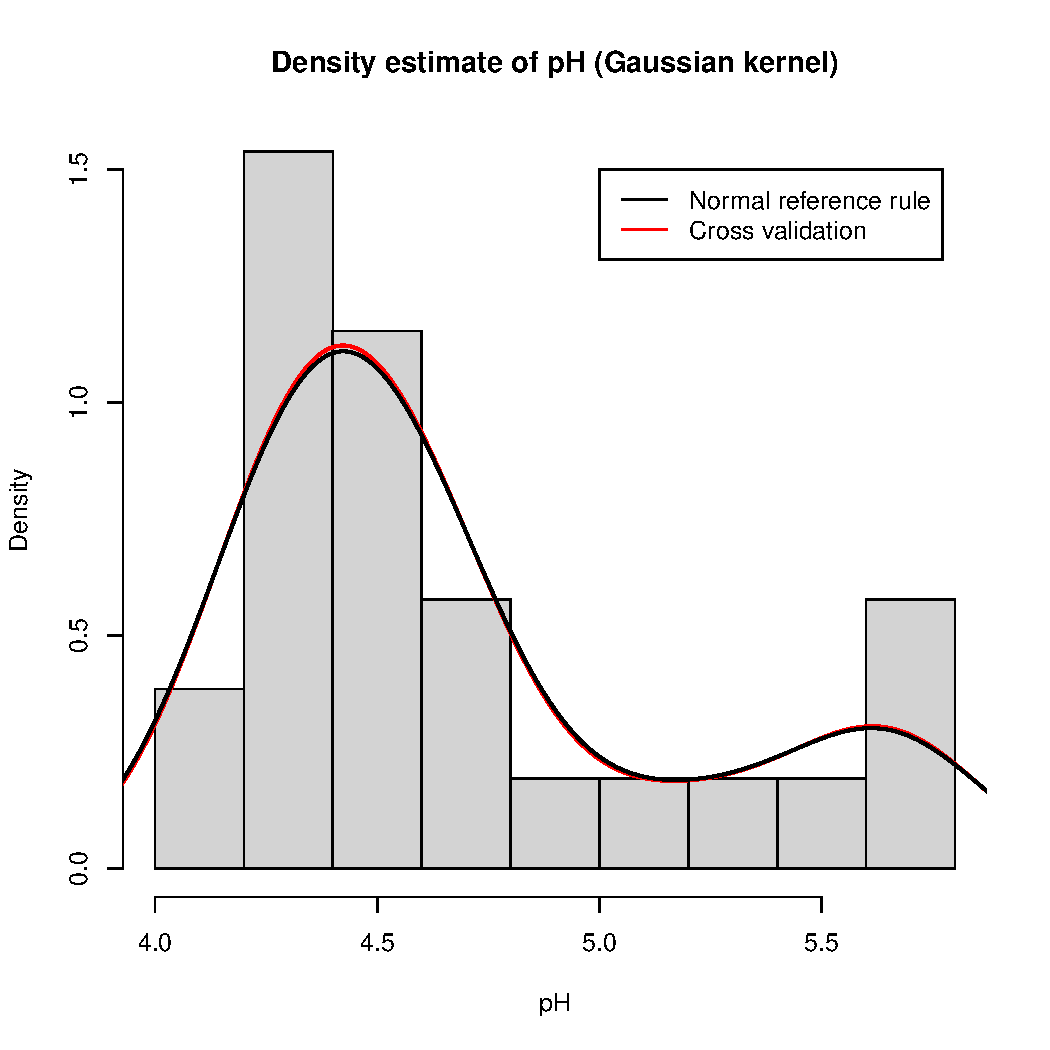
\includegraphics[width=\textwidth, page = 1]{acid-rain.pdf}
             \caption{Gaussian kernel}
         \end{subfigure}
         \hfill
         \begin{subfigure}[b]{0.45\textwidth}
             \centering
             \includegraphics[width=\textwidth, page = 2]{acid-rain.pdf}
             \caption{Epanechnikov kernel}
         \end{subfigure}
         \hfill
         \begin{subfigure}[b]{0.45\textwidth}
             \centering
             \includegraphics[width=\textwidth, page = 3]{acid-rain.pdf}
             \caption{Rectangular kernel}
         \end{subfigure}
         \begin{subfigure}[b]{0.45\textwidth}
             \centering
             \includegraphics[width=\textwidth, page = 4]{acid-rain.pdf}
             \caption{Triangular kernel}
         \end{subfigure}
        \caption{Kernel density estimates of pH.}
        \label{fig:kernel_density_estimates}
    \end{figure}


\end{document}
